\documentclass[a4paper,12pt]{article}
\author{Adam Ilyas}
\title{
CS-E5740 Complex Networks, \\
Answers to exercise set 1
}

\usepackage{a4wide}
\usepackage{amsfonts}
\usepackage{verbatim}
\usepackage{amsmath}
\usepackage{amsfonts}
\usepackage{graphicx}
\usepackage[english]{babel}
\usepackage{listings}

\begin{document}
\vspace{8pt}

\maketitle

\section{Basic network properties}

\begin{figure}[!ht]
	\begin{center}
    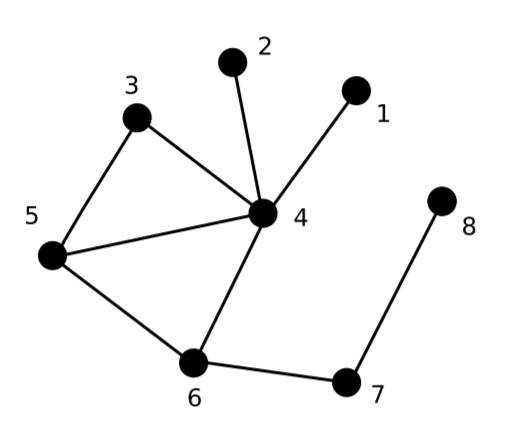
\includegraphics[scale=0.33]{graph_ex_1.png}
    \caption{The graph for exercise 1.}
	\label{fig:graph1}
	\end{center}
\end{figure}

\subsection*{a. Adjacency matrix}
A network data structure in the form of a matrix used to represent a
graph
\[
  a_{ij}=\begin{cases}
               1 \quad if \quad (j,i) \in E\\
               0 \quad if \quad (j,i) \notin E
            \end{cases}
\]
Hence, the adjacency matrix for the graph in figure 1 is as follows:

	$$
	\begin{bmatrix} 
		0&0&0&1&0&0&0&0\\
		0&0&0&1&0&0&0&0\\
		0&0&0&1&1&0&0&0\\
		1&1&1&0&1&1&0&0\\
		0&0&1&1&0&1&0&0\\
		0&0&0&1&1&0&1&0\\
		0&0&0&0&0&1&0&1\\
		0&0&0&0&0&0&1&0
	\end{bmatrix}$$

\subsection*{b. Edge density}
The edge density of a network is the fraction of edges out of possible edges:

$$\rho = \frac{m}{{N\choose 2}} = \frac{2m}{N(N-1)}$$
where $m$ is the number of edges and $N$ is the number of vertices.
\newline Total possible edges is
$\frac{N(N-1)}{2}$ which is $1 + 2 + 3 ... + (N-2) + (N-1)$
\newline \newline
The edge density $\rho$ of graph 1 is $\frac{18}{56}$ = 0.321

\subsection*{c. Degree and Degree Distribution}
The degree $k_i$ of vertex $v_i$ is the number of edges it is incident to.\newline
\begin{table}[h]
\centering
\begin{tabular}{c|c}
Vertices & Degree\\
\hline
1 & 1\\
2 & 1\\
3 & 2\\
4 & 5\\
5 & 3\\
6 & 3\\
7 & 2\\
8 & 1
\end{tabular}
\end{table}
\break
The degree distribution $P(k)$ is the probability that the degree of a randomly chosen node is $k$.
$$P(k) = \frac{N_k}{N}$$
where $N_k$ is the number of nodes of degree $k$.\newline\newline
The degree distribution $P(k)$ of graph 1: 
\begin{table}[h]
\centering
\begin{tabular}{c|c}
k & P(k)\\
\hline
1 & 0.375\\
2 & 0.25\\
3 & 0.25\\
4 & 0\\
5 & 0.125
\end{tabular}
\end{table}
\subsection*{d. The mean degree $\langle k \rangle$ of the graph}
The average degree $\langle k \rangle$ of a network is:
$$\langle k \rangle = \sum_{i}\frac{k_i}{N} = \frac{2m}{N}$$
where $m$ is the number of edges, $N$ is the number of vertices, $k_i$ is the degree for vertice $i$\newline\newline
The mean degree $\langle k \rangle$ for graph 1 is 2.25

\subsection*{e. The diameter $d$ of the graph.}
Diameter $d$ is the largest distance in the network (It is the shortest distance between the two most distant nodes in the network.): $\max_{i,j \in V}d_{ij}$\newline\newline Diameter of graph 1: 4

\subsection*{f. The clustering coefficient $C_i$}
The clustering coefficient $C_i$ for each node $i \in V$ that has degree $k_i > 1$. For nodes with $k_i$ = 0,1, we define $C_i$ = 0.\newline\newline
Clustering coefficient defined for node i as the fraction of edges between
its neighbours out of possible edges between its neighbours:
$$C_i = \frac{E_i}{{k_i\choose2}} = \frac{2E_i}{k_i(k_i - 1)}$$
\begin{table}[h]
\centering
\begin{tabular}{c|c}
Vertices & $C_i$\\
\hline
1 & 0\\
2 & 0\\
3 & 1\\
4 & 0.2\\
5 & 0.66\\
6 & 0.33\\
7 & 0\\
8 & 0 
\end{tabular}
\end{table}
\newline
Average clustering coefficient (averaged over all nodes) is $c = \frac{1}{N}\sum_{i}c_i = \frac{2.2}{8} = 0.275$

\section{Computing network properties programmatically}

\subsection*{a. Load the edge list and visualize the network}
\begin{lstlisting}
# python3
import networkx as nx

fn = 'karate_club_network_edge_file.edg'
graph = nx.read_weighted_edgelist(fn)

fig, ax = plt.subplots(figsize=(12, 8))
nx.draw(graph, with_labels=True)
ax.set_title('The Karate Club network')
\end{lstlisting}
Network:
\begin{figure}[!ht]
	\begin{center}
    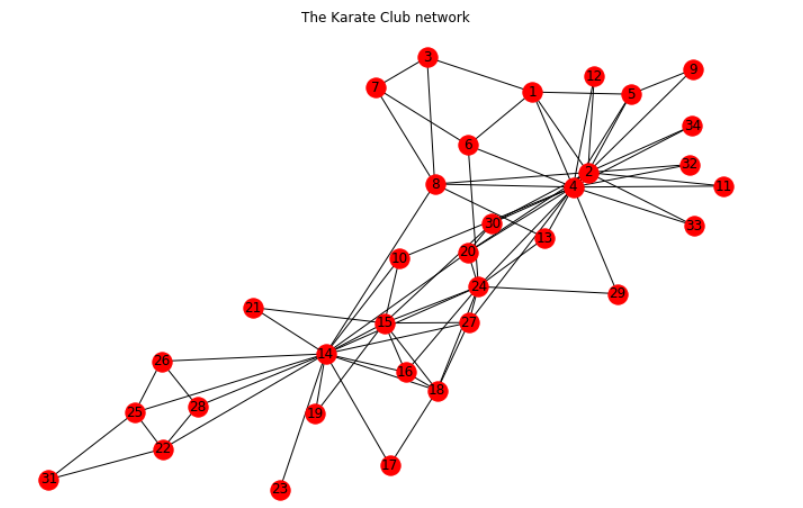
\includegraphics[scale=0.8]{graph_karate.png}
    \caption{Karate Club Network graph}
	\label{fig:graph2}
	\end{center}
\end{figure}

\subsection*{b. Calculate the edge density of the karate club network.}
First, write your own code without using networkx.density and then compare your result to the output of networkx.density (the corresponding NetworkX function).
\begin{lstlisting}
m = graph.number_of_edges()
n = graph.number_of_nodes()
density = 2*m/(n*(n-1))
\end{lstlisting}
Edge Density: 0.13903743315508021

\subsection*{c. Calculate the average clustering coefficient}
Calculate the average clustering coefficient with your own algorithm and compare it to the output of the corresponding NetworkX function.
\begin{lstlisting}
def clustering_coefficient(node):
    n_links = 0
    neighbours = list(graph.neighbors(node))
    k = len(neighbours)
    if k<2:
        return 0
    for neighbour_node in neighbours:
        for other_node in neighbours:
            if graph.has_edge(neighbour_node, other_node):
                n_links += 1
    
    n_links = n_links/2 # double counting

    return 2 * n_links / (k * (k-1))
    
# apply function to every single node
all_nodes = list(graph.nodes)
node_ls = {}
for node in all_nodes:
    cc = clustering_coefficient(node)
    node_ls[node] = {"coefficient": cc}
    
sum([node_ls[node]["coefficient"] for node in node_ls])/ len(node_ls) 
\end{lstlisting}
Average Clustering Coefficient:  0.5706384782076824

\subsection*{d. Calculate the Degree Distribution}
Calculate the degree distribution P(k) and the complementary cumulative degree distribution-CDF(k) of the network. Visualize the distributions using matplotlib.pyplot. 

\begin{table}[h]
\centering
\begin{tabular}{c|c}
Degree & Degree Distribution (\%)\\
\hline
1 & 0.029\\
2 & 0.324\\
3 & 0.176\\
4 & 0.176\\
5 & 0.088\\
6 & 0.059\\
9 & 0.029\\
10 & 0.029\\
12 & 0.029\\
16 & 0.029\\
17 & 0.029
\end{tabular}
\end{table}
\begin{figure}[h!]
	\begin{center}
    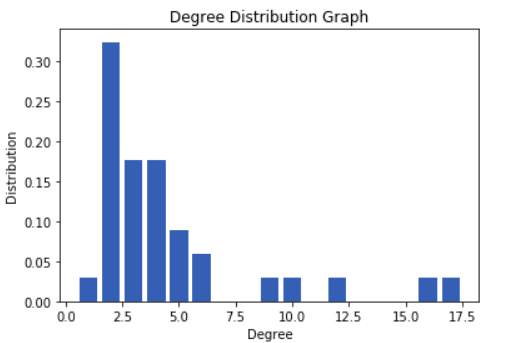
\includegraphics[scale=0.8]{graph_degree_distribution.png}
    \caption{Degree Distribution Graph}
	\end{center}
\end{figure}
\begin{figure}[h!]
	\begin{center}
    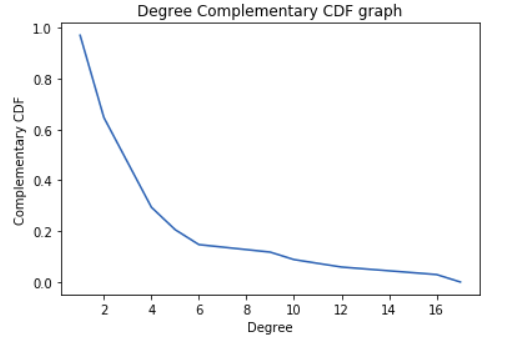
\includegraphics[scale=0.8]{graph_ccdf.png}
    \caption{Degree Complementary CDF graph}
	\end{center}
\end{figure}

\clearpage

\subsection*{e. Calculate the average shortest path length}
\begin{lstlisting}
length = nx.average_shortest_path_length(graph)
\end{lstlisting}
Average shortest path length:  2.408199643493761

\subsection*{f. Create a scatter plot of $C_i$ as a function of $k_i$.}
Using matplotlib.pyplot library
\begin{figure}[h!]
	\begin{center}
    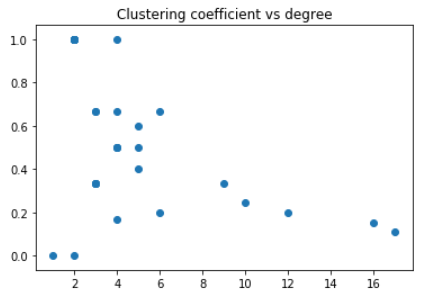
\includegraphics[scale=0.8]{graph_scatter.png}
    \caption{$C_i$ as a function of $k_i$}
	\end{center}
\end{figure}

\section{Number of walks}

\subsection*{a. Draw the induced subgraph G*}
where G* is induced by the the vertices V* = $\{1…4\}$ of network visualized in Figure 1. Calculate by hand the number of walks of length two between all node pairs $(i,j), i, j \in \{1...4\}$; a link can be travelled in both directions and the walk can visit a node multiple times. Remember to consider also walks, where $i = j$. Then, compute the matrix $A^2$ (you may do this also using a computer), where A is the adjacency matrix of the network G*. Compare your results; what do you notice? 

\begin{figure}[h]
	\begin{center}
    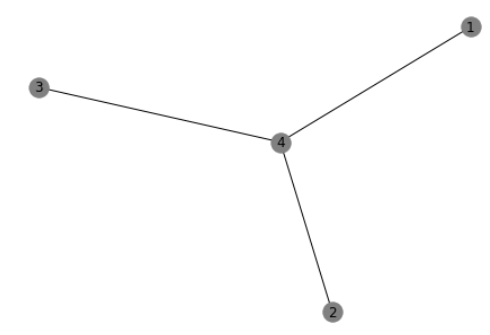
\includegraphics[scale=0.5]{induced.png}
    \caption{Induced subgraph G*}
	\end{center}
\end{figure}

\begin{table}[h]
\centering
\begin{tabular}{c|c|c|c}
Node 1 & Node 2 & Node 3 & Node 4\\
\hline
1-4-1 & 2-4-2 & 3-4-3 & 4-1-4\\
1-4-2 & 2-4-1 & 3-4-1 & 4-2-4\\
1-4-3 & 2-4-3 & 3-4-2 & 4-3-4\\
\end{tabular}
\end{table}

The adjacency matrix for the sub graph in figure 2 is as follows:

	$$
	A = \begin{bmatrix} 
		0&0&0&1\\
		0&0&0&1\\
		0&0&0&1\\
		1&1&1&0\\
	\end{bmatrix} \quad
	A^2 = \begin{bmatrix} 
		1&1&1&0\\
		1&1&1&0\\
		1&1&1&0\\
		0&0&0&3\\
	\end{bmatrix}
	$$
$A^2_{ij}$ refers to the number of walks from $i$ to $j$ where the length = 2. E.g. $A^2_{11} = 1$ where their is only 1 possible walk with length 2, from node 1 to 1 (1-4-1). For $A^2_{44} = 3$ there are 3 such walks, as shown the table above

\subsection*{b. Compute the number of walks of length 3 from node 3 to 4} Compute the number of walks of length three from node 3 to node 4 in G*. Then, starting from matrices $A^2$ and $A$, compute by hand the value of $(A^3)_{3,4}$ showing also the intermediate steps for computing the matrix element.
\begin{table}[h]
\centering
\begin{tabular}{c}
Walks\\
\hline
3-4-3-4\\
3-4-1-4\\
3-4-2-4
\end{tabular}
\end{table}

	\[A^3 = 
	\begin{bmatrix} 
		1&1&1&0\\
		1&1&1&0\\
		1&1&1&0\\
		0&0&0&3
	\end{bmatrix}
	\cdot
	\begin{bmatrix} 
		0&0&0&1\\
		0&0&0&1\\
		0&0&0&1\\
		1&1&1&0
	\end{bmatrix}	
	= 
	\begin{bmatrix} 
		0&0&0&3\\
		0&0&0&3\\
		0&0&0&3\\
		3&3&3&0
	\end{bmatrix}\]
From the matrix above, $(A^3)_{3,4} = 3$
\subsection*{c. Proving}
Now, let's consider a general network with adjacency matrix A. \textbf{Show} that the element $(A^m)_{ij}, m \in \mathbb{N}$  corresponds to the number of walks of length m between nodes i and j. \\ \textit{Hint:} Make use of mathematical induction: show that the  statement holds for general $m$ and prove that it holds for $m+1$.\\\\\textbf{Base case}\\
For $m=1$ the statement holds, for $A^1$ is the adjacency matrix.\\\\
\textbf{Inductive step}\\
For a general $m$, first we assume $a_{ij}^{(m)}$ gives the number of walks of length m\\\\
For $m+1$, 
\begin{equation}
\begin{split}
(A^{m+1})_{ij} & = (A^m \cdot A)_{ij} \\
& = \sum_{l=1}^{N} (a_{il}^m \times a_{lj})\\
& = a_{ij}^{m+1}
\end{split}
\end{equation}
\end{document}
